% --------------------------------------------------------------
% This is all preamble stuff that you don't have to worry about.
% Head down to where it says "Start here"
% --------------------------------------------------------------
 
\documentclass[12pt]{article}
 
\usepackage[margin=1in]{geometry} 
\usepackage{amsmath,amsthm,amssymb,algpseudocode,listings}
\usepackage{color}
\usepackage{DejaVuSansMono} 
\usepackage{setspace}
\usepackage{parskip}
\usepackage{graphicx}


\definecolor{Code}{rgb}{0,0,0}
\definecolor{Decorators}{rgb}{0.5,0.5,0.5}
\definecolor{Numbers}{rgb}{0.5,0,0}
\definecolor{MatchingBrackets}{rgb}{0.25,0.5,0.5}
\definecolor{Keywords}{rgb}{0,0,1}
\definecolor{self}{rgb}{0,0,0}
\definecolor{Strings}{rgb}{0,0.63,0}
\definecolor{Comments}{rgb}{0,0.63,1}
\definecolor{Backquotes}{rgb}{0,0,0}
\definecolor{Classname}{rgb}{0,0,0}
\definecolor{FunctionName}{rgb}{0,0,0}
\definecolor{Operators}{rgb}{0,0,0}
\definecolor{Background}{rgb}{0.98,0.98,0.98}

\lstnewenvironment{python}[1][]{
\lstset{
numbers=left,
numberstyle=\ttfamily,
numbersep=1em,
xleftmargin=1em,
framextopmargin=2em,
framexbottommargin=2em,
showspaces=false,
showtabs=false,
showstringspaces=false,
frame=l,
tabsize=4,
% Basic
basicstyle=\ttfamily\small\setstretch{1},
backgroundcolor=\color{Background},
language=Python,
% Comments
commentstyle=\color{Comments}\slshape,
% Strings
stringstyle=\color{Strings},
morecomment=[s][\color{Strings}]{"""}{"""},
morecomment=[s][\color{Strings}]{'''}{'''},
% keywords
morekeywords={import,from,class,def,for,while,if,is,in,elif,else,not,and,or,print,break,continue,return,True,False,None,access,as,,del,except,exec,finally,global,import,lambda,pass,print,raise,try,assert},
keywordstyle={\color{Keywords}\bfseries},
% additional keywords
morekeywords={[2]@invariant},
keywordstyle={[2]\color{Decorators}\slshape},
emph={self},
emphstyle={\color{self}\slshape},
%
}}{}

\newcommand{\N}{\mathbb{N}}
\newcommand{\Z}{\mathbb{Z}}
 
\newenvironment{theorem}[2][Theorem]{\begin{trivlist}
\item[\hskip \labelsep {\bfseries #1}\hskip \labelsep {\bfseries #2.}]}{\end{trivlist}}
\newenvironment{lemma}[2][Lemma]{\begin{trivlist}
\item[\hskip \labelsep {\bfseries #1}\hskip \labelsep {\bfseries #2.}]}{\end{trivlist}}
\newenvironment{exercise}[2][Exercise]{\begin{trivlist}
\item[\hskip \labelsep {\bfseries #1}\hskip \labelsep {\bfseries #2.}]}{\end{trivlist}}
\newenvironment{problem}[2][Problem]{\begin{trivlist}
\item[\hskip \labelsep {\bfseries #1}\hskip \labelsep {\bfseries #2.}]}{\end{trivlist}}
\newenvironment{question}[2][Question]{\begin{trivlist}
\item[\hskip \labelsep {\bfseries #1}\hskip \labelsep {\bfseries #2.}]}{\end{trivlist}}
\newenvironment{corollary}[2][Corollary]{\begin{trivlist}
\item[\hskip \labelsep {\bfseries #1}\hskip \labelsep {\bfseries #2.}]}{\end{trivlist}}


\lstset{basicstyle=\footnotesize\ttfamily,breaklines=true}
\lstset{framextopmargin=50pt,frame=bottomline}

\begin{document}
 
% --------------------------------------------------------------
%                         Start here
% --------------------------------------------------------------
 
\title{Homework 4 \& 5}%replace X with the appropriate number
\author{Jeremy Wright\\ %replace with your name
CSE598 - Analysis of Algorithms} %if necessary, replace with your course title
 
\maketitle
\begin{problem}{1}
    Show how to multiple the complex numbers $a+bj$ and$c+dj$ using only three
    real multiplications\dots

    Given: 
        \begin{align*}
        R+jI &= (a+jb)\cdot(c+jd) \\
        &= (ac - bd) + j(bc + ad)
    \end{align*}

    A common pattern in Digital Signal Processing is to break out the operations
    into 3 constants.
    \begin{align*}
        \label{eq:components}
        k_1 &= a(c + d) &= ac + ad \\
        k_2 &= d(a + b) &= ad + bd \\
        k_3 &= c(b - a) &= bc - ac \\
    \end{align*}
    From these we can define the Real part as
    \begin{align*}
        \Re &= k_1 - k_2 \\
            &= ac + ad - (ad + bd) \\
            &= ac + ad - ad - bd \\
            &= ac - bd \\
    \end{align*}
    The Imaginary Part as
    \begin{align*}
        \Im &= k_1 + k_3            \\
            &= ac + ad + bc - ac    \\
            &= ab + bc
    \end{align*}

    In Python we can clearly see this uses only 3 multiplications.
    \begin{python}
        def complex_mul(a, b, c, d):
            k1 = a(c + d)
            k2 = d(a + b)
            k3 = c(b - a)
            return (k1 - k2) + (k1 - k3)*j
    \end{python}
\end{problem}

\begin{problem}{2}
Consider in the closest pair of points problem, splitting the points along
$ \frac{n}{4}$ and $\frac{3n}{4}$. Is the complexity still $O(n lg n)$? Yes

Proof:

Consider the base case $ n >= 4$:
\begin{equation*}
    T(n) = T(\frac{n}{4}) + T(\frac{3n}{4}) + n
\end{equation*}
Substitute $n lg n$
\begin{align*}
    T(n) =& T(\frac{n}{4}) + T(\frac{3n}{4}) + n\\
    T(n) \le& c \frac{n}{4} \log_2{\frac{n}{4}}    + c \frac{3n}{4}\log_2{\frac{3n}{4}} + cn\\
    \le& c \left( \frac{n}{4} \log_2{n} - \frac{n}{4} \log_2{4} \right)
    + c \left(\frac{3n}{4} \log_2{3n} - \frac{3n}{4} \log_2{4} \right) + cn \\
    \le& c \left( \frac{n}{4} \log_2{n} - \frac{2n}{4} \right)  + c \left( \frac{3n}{4} \log_2{3n} - \frac{3n\cdot2}{4} \right) + cn \\
    \le& c\left(\frac{n}{4} \log_2{n} - \frac{1}{2}n\right)   + c \left(\frac{3n}{4} \log_2{3} + \frac{3n}{4} \log_2{n} - \frac{3n}{2}\right) + cn\\
    \le& c\frac{n}{4} \log_2{n} - \frac{1}{2}cn + \frac{3nc}{4} \log_2{n} - cn
    + cn\\
    \le& c\frac{n}{4} \log_2{n} + \frac{3cn}{4}\log_2{n} \\
    \le& cn\log_2{n}
\end{align*}
Intuitively this makes sense because we are still dividing the space into some
log relatable ratio for each subproblem. 

Consider dividing the space into $\sqrt{n}$ and $n-\sqrt{n}$. This problem will
not remain at $n \log_2{n}$ since the division of the space is not an even
recurrence. Instead there is a linear adjustment in the form of $n - \dots$
\begin{align*}
    T(n) &= T(n^{\frac{1}{2}}) + T(n-n^{\frac{1}{2}}) + nc\\
    \le& n^{\frac{1}{2}} \log_2{n^{\frac{1}{2}}} + \left(n-
    n^{\frac{1}{2}}\right) \log_2\left(n - n^{\frac{1}{2}}\right) c + cn
    \dots
\end{align*}
Eventually we get to where we cannot resolve the logs with the roots.  So let's
try a greater complexity: $n^2$
\begin{align*}
    \le& \left( n^{\frac{1}{2}} \right)^2 + \left( n - n^\frac{1}{2} \right)^2
    + nc\\
    \le& n + n^2 - n + nc\\
    \le& n^2 + n(1 - 1 + 1)c\\
    \le& n^2 + nc\\
    \le& \lim_{n\to \infty}\left(n^2 + nc\right)\\
    \le& cn^2
\end{align*}
Thus by adding an irregular division to the sub problems we increase the
complexity to recombine those subproblems.
\end{problem}
\begin{problem}{5.1}
    Find the median of two databases. Use at most $O(log_2{n})$ queries.

    To achieve this complexity target we must do at most a recurrence of 
    \begin{equation}
        T(n) = T(\frac{n}{2}) + c
    \end{equation}
    With a Base case of $T(1) = 1$, since a median of a single element is
    itself $\therefore$
    \begin{equation}
        T(n) = T( \frac{n}{2}) + O(1)
    \end{equation}
     Intuitively, this represents an algorithm which divides the input into
     2 subproblems, considers one side and spends a constant amount of time at
       each step.
    Such an algorithm may be implemented in Python:
    \begin{python}
import numpy

def median( ns ):
    l = len(ns)
    if l % 2 == 0:
        return (ns[l/2] + ns[(l/2)-1])/2.0
    else:
        return ns[l/2]


def find_median(a, b):
    l = len(a)
    if l == 1:
        return (median(a) + median(b)) / 2
    if l == 2:
        return ( max(a[0], b[0]) + min(a[1], b[1]) ) / 2

    ma = median(a)
    mb = median(b)

    if ma == mb:
        return ma
    
    if ma < mb:
        if l % 2 == 0:
            return find_median(a[l/2:], b[:l/2])
        else:
            return find_median(a[l/2:], b[:(l/2)+1])
    else:
        if l % 2 == 0:
            return find_median(a[l/2-1:], b[l/2-1:])
        else:
            return find_median(a[:(l/2)+1], b[(l/2):])

import random
for i in range(10):
    a = [random.randint(0,10) for r in xrange(10)]
    b = [random.randint(0,10) for r in xrange(10)]
    c = a + b

    a.sort()
    b.sort()
    c.sort()
    print a, b, c
    if median(c) == find_median(a,b):
        print "PASS"
    else:
        print "FAIL"
    \end{python}
This algorithm leverages subranges (called splices in Python).  Lines 12 - 16
describe the various end conditions and base cases.  Once complete, one must
start the merging of each subrange. If the median of list a is less than the
median of list b, then the median of the entire set must lie in the right half
of list a, or the left half of list b.

Conversely, if list b's median is greater, then the median must lie in the left
half of a.

\begin{problem}{5.5 (graduate)}
Design an algorithm which finds the visible lines in $O(n lg n)$ time. 

The brute force of this problem, would be to compare the intersections of all
lines, sorting the y values, and dropping the invisible lines. This however
results in $\Omega(n^2)$.

The algorithm must then divide the input in such a way that it doesn't have to
enumerate \emph{all} intersections.

Consider:
\begin{enumerate}
    \item Sort the list of lines by their slope.
    \item Add line to the visible list.
    \item Starting at the beginning of the list, find all intersections with
        this line to the lines to its right in the list.
    \item Take the line who's intersection is greatest. Add this
 line to the visible list.
 \item Now repeat with this line, find all intersections with lines to it's
     right.
     \end{enumerate}
\end{problem}

This algorithm sorts in O(n lg n) using something like Merge Sort.
Then at each step it only considers lines to it's right in the sorted slope
list. Each line with a greater y value gets added to the visible list, and
becomes the next line to consider, never considering lines behind us, or already
in the visible list. In this way we beat $n^2$ time.
\end{problem}

\begin{problem}{6.3}
    Given an ordered graph G, find the length of the longest path that begins at A and ends at E.
    
    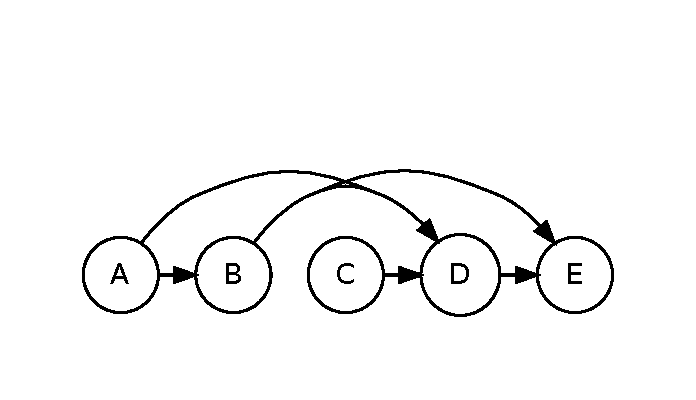
\includegraphics{6_3a.pdf}

    The given algorithm is a greedy algorithm and always chooses the nearest
    node hoping to get to the end as late as possible. However in the example
    below, the blue path is the longest path, with length 4, wile the red path
    is length 2. The greedy algorthm does not see beyond node 2, and incorrectly
    follows the red path.

    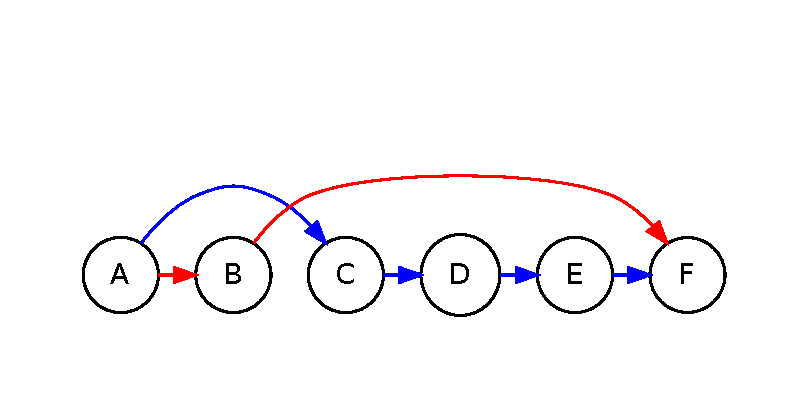
\includegraphics{6_3b.pdf}
    
    Dynamic programming can help here by ``carefully'' evaulating all possible
    paths. First a few constraints. The graph must be acyclic,, and have
    a topolocial sort, which by definition it does. 

    Next we use a 5 step process. 
    \begin{enumerate}
        \item Define sub problems.
        \item Guess a metric to minimize/maximize.
        \item Relate the sub problems (recurrence)
        \item Solve the recurrence, and memoize the algorithm.
        \item Recombine the subproblems (verify the original problem gets
            solved.)
    \end{enumerate}
     
    1. Define sub problems. Consider the incomming edges to the final node. The
       longest path must be one of those edges, so use dynamic programming to
       carefully try them all.
    
    2. Guess the last edge comming into the final node v. Next recurrsively
       find the longest path to u and add the longer path to v. 
    
    3. Relate sub problems. Define a function $\delta(s,v)$ which is the
       length of the edge from the path from s to v. 
       \begin{equation}
           \delta(s,v) = max\{ \delta(s, u) + (u \to v).\text{weight } \forall
               \text{ Edges = u} \}
       \end{equation}
        Time per subproblem is $\delta(s,v) = indegree(v)$. 
        Total time
        \begin{equation}
            \sideset{}{}\sum_{v \in G}indegree(v) = \theta(E + V)
        \end{equation}

\end{problem}
\begin{problem}{6.5}
    Consider the string ilovemywife.

    Consider all the suffixes of this string.

    define a recurrence $Q(s,f)$ where s is the starting index, and f is the
    closed finish index. $Q(s,f)$ returns the quality for that string. We want
    to maximze the quality of the sentence. So lets ``carefully'' try all
    suffixes.

    1. Subproblems. suffixes of works words[i:] (in python notation).\\
        \# number of subproblems is n in the number of letters

    2. Guess where to start the second word.\\
        \# number of choices (n - 1) since the first letter must be at the first
        word.

    3. Recurrence
        \begin{equation}
            word(i) = max\{ word(j) + Q(i, j) \text{ for j in range(i+1,
            n + 1)}\}
        \end{equation}
    4. Total runnign time is time / subproblem * number of problems
       = $\theta(n^2)$.

    5. Original subproblem is the maximum quality starting from the first
       character i.e. $word(0)$. 
\end{problem}
\end{document}
